% dibuix_cilindre_1.tex
\documentclass{standalone}
\usepackage{tikz}
\usetikzlibrary{arrows.meta, decorations.markings, decorations.pathmorphing}

\begin{document}

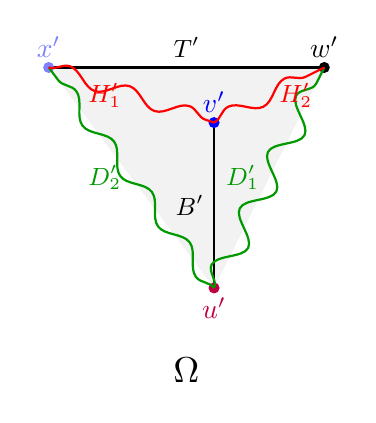
\begin{tikzpicture}[
    identified_edge/.style={
        decoration={
            markings,
            mark=at position 0.5 with {\arrow{Latex}}
        },
        postaction={decorate}
    },
    edge_label/.style={midway, auto, font=\small}
]

\def\squaresize{3.5}
\fill[gray!10] (0,\squaresize) -- (\squaresize,\squaresize) -- (0.6 * \squaresize, 0.2 * \squaresize) -- cycle;
\draw[thick] (0, \squaresize) -- node[edge_label, above] {$T'$} (\squaresize,\squaresize);
\draw[thick] (0.6 * \squaresize, 0.2 * \squaresize) -- node[edge_label, left] {$B'$} (0.6 * \squaresize,0.8 * \squaresize);

\node[scale=1.3] at (0.5 * \squaresize,-0.1*\squaresize) {$\Omega$};
\fill[purple] (0.6 * \squaresize, 0.2 * \squaresize) circle (2pt) node[below] {$u'$};
\fill[blue!50] (0,\squaresize) circle (2pt) node[above] {$x'$};
\fill[blue] (0.6 * \squaresize,0.8 * \squaresize) circle (2pt) node[above] {$v'$};
\fill[black] (\squaresize,\squaresize) circle (2pt) node[above] {$w'$};

\draw[thick, green!60!black, decoration={snake, amplitude=1mm, segment length=8mm}, decorate] (0.6 * \squaresize, 0.2 * \squaresize) -- node[edge_label, left] {$D_2'$} (0,\squaresize);
\draw[thick, green!60!black, decoration={snake, amplitude=1.6mm, segment length=8mm}, decorate] (0.6 * \squaresize, 0.2 * \squaresize) -- node[edge_label, left] {$D_1'$} (\squaresize,\squaresize);

\draw[thick, red, decoration={snake, amplitude=1mm, segment length=8mm}, decorate] (0,\squaresize) -- node[edge_label, left] {$H_1'$} (0.6 * \squaresize,0.8 * \squaresize);
\draw[thick, red, decoration={snake, amplitude=1mm, segment length=8mm}, decorate] (0.6 * \squaresize,0.8 * \squaresize) -- node[edge_label, right] {$H_2'$} (\squaresize,\squaresize);




\end{tikzpicture}

\end{document}